%!TEX root = ../main.tex

\newpage

\chapter{Entwurf} %  (fold)
\label{cha:entwurf}

\section{Grober Entwurf (Architektur)}
\label{sec:groberentwurf}

\section{Technologien}
\label{sec:technologien}

	\begin{itemize}	
		\item Bluetooth
		\item SQL Datenbank
		\item JAVA (Android)
	\end{itemize}
\section{Detaillierter Entwurf}
\label{sec:detaillierterentwurf}

\subsection{ESP: Befehle}
\label{sec:espbefehle}

Nachrichten werden als JSON-Maps (in UTF8) kodiert und folgen alle dem selben Format.

Für unverschlüsselte Nachrichten ist das Format:

*\{"cmd": "der Befehl", "user": "die User-ID", "argument": "weitere Werte", ...\}
*

Das "cmd"-Feld ist verpflichtend und enthält den Namen des Befehls. Die meisten Nachrichten benötigen auch ein "user"-Feld mit der User-ID. Eventuelle weitere Argumente werden als weitere Felder in der Map gesendet.

Für verschlüsselte Nachrichten wird die Nachricht in einen Wrapper gepackt:

*
\{"msg": "verschlüsselte JSON-Nachricht", "user": "die User-ID"\}
*

Der Key zum Entschlüsseln ist mit der User-ID verbunden und wird benutzt, um die Nachricht in "msg" zu ver-/entschlüsseln. Die entschlüsselte Nachricht ist ein normaler Befehl der Form `{"cmd": ...}`.

Momentan unterstützt der ESP noch keine verschlüsselten Nachricht.

\subsubsection{ Allgemeine Befehle}

\paragraph{ test (USER): Dummy-Befehl, der nichts macht}

JSON-Beispiel:

*
\{"cmd": "test"\}
*

\paragraph{ init\_user (USER): als neuer Benutzer registrieren und eine User-ID erhalten}

- name: str

JSON-Beispiel:

*
\{"cmd": "init\_user", "name": "test-user"\}

--> \{"user": 100\}
*

\paragraph{ reset (ADMIN): die Maschine zurücksetzen}

- user: User

Der Befehl entfernt den aktuellen Cocktail und setzt die Maschine wieder in den normalen Zustand zurück. Das ist nur beim Testen notwendig.

JSON-Beispiel:

*
{"cmd": "reset", "user": 0}
*

\paragraph{ reset\_error (ADMIN): gespeicherten Fehler zurücksetzen}

- user: User

Der Befehl entfernt den aktuellen Fehler und macht im normalen Betrieb weiter. Das kommt meistens nur vor, wenn ein Rezept ein Problem hatte und die Maschine das Problem nicht beheben konnte.

JSON-Beispiel:

*
{"cmd": "reset\_error", "user": 0}
*

\paragraph{ clean (ADMIN): reinigt die Maschine}

- user: User

JSON-Beispiel:

*
{"cmd": "clean", "user": 0}
*

\paragraph{ restart (ADMIN): startet die Maschine neu}

- user: User

JSON-Beispiel:

*
{"cmd": "restart", "user": 0}
*

\paragraph{ factory\_reset (ADMIN): setzt alle Einstellungen zurück}

- user: User

JSON-Beispiel:

*
{"cmd": "factory\_reset", "user": 0}
*

\subsubsection{ Rezepte definieren}

\textbf{ define\_recipe (USER): definiert ein neues Rezept}

- user: User
- name: str
- ingredients: List[Tuple[str, float]]

JSON-Beispiel:

*
\{"cmd": "define\_recipe", "user": 0, "name": "radler", "ingredients": [["beer", 250], ["lemonade", 250]]\}
*

\paragraph{ edit\_recipe (USER): editiert ein Rezept}

- user: User
- name: str
- ingredients: List[Tuple[str, float]]

JSON-Beispiel:

*
{"cmd": "edit\_recipe", "user": 0, "name": "radler", "ingredients": [["beer", 250], ["lemonade", 250]]}
*

\paragraph{ delete\_recipe (USER): löscht ein Rezept}

- user: User
- name: str

JSON-Beispiel:

*
\{"cmd": "delete\_recipe", "user": 0, "name": "radler"\}
*

\subsubsection{ Rezepte machen}

Der Ablauf um ein Rezept zu machen ist:

1. Das Rezept mit `queue\_recipe` in Auftrag geben. Das Rezept kommmt in die Warteschlange. Die aktuellen Benutzer in der Warteschlange können mit dem Status `user` ausgelesen werden.

2. Wenn die Maschine bereit ist, wird der Status `state` auf `waiting for container` gesetzt. Sobald ein Gefäß in der Maschine ist, kann das Rezept mit dem Befehl `start\_recipe` gestartet werden.

3. Wenn das Rezept fertig ist, wird der Status `state` auf `cocktail done` gesetzt. Der Cocktail kann entnommen werden. Das Rezept wird mit `take\_cocktail` beendet.

4. Die Maschine beginnt dann mit dem nächsten Rezept in der Warteschlange.


\paragraph{ queue\_recipe (USER): gibt ein Rezept in Auftrag}

- user: User
- recipe: str

JSON-Beispiel:

*
\{"cmd": "queue\_recipe", "user": 8858, "recipe": "radler"\}
*

\paragraph{ start\_recipe (USER): fängt das Rezept an, wenn die Maschine bereit ist}

- user: User

JSON-Beispiel:

*
\{"cmd": "start\_recipe", "user": 8858\}
*

\paragraph{ cancel\_recipe (USER): bricht das aktuelle Rezept ab}

- user: User

JSON-Beispiel:

*
\{"cmd": "cancel\_recipe", "user": 483\}
*

\paragraph{ take\_cocktail (USER): gibt Bescheid, dass der Cocktail entnommen wurde}

- user: User

JSON-Beispiel:

*
\{"cmd": "take\_cocktail", "user": 483\}
*

\paragraph{ add\_liquid (USER): fügt Flüssigkeit zum aktuellen Rezept hinzu}

- user: User
- liquid: str
- volume: float

JSON-Beispiel:

*
\{"cmd": "add\_liquid", "user": 0, "liquid": "water", "volume": 30\}
*

\subsubsection{ Pumpen}

\paragraph{ define\_pump (ADMIN): fügt Pumpe zu ESP hinzu}

- user: User
- liquid: str
- volume: float
- slot: int

JSON-Beispiel:

*
\{"cmd": "define\_pump", "user": 0, "liquid": "water", "volume": 1000, "slot": 1\}
*

\paragraph{ define\_pumps (ADMIN): fügt mehrere Pumpe zu ESP hinzu}

- user: User
- liquid: str
- volume: float
- quantity: int

JSON-Beispiel:

*
\{"cmd": "define\_pumps", "user": 0, "liquid": "water", "volume": 0, "quantity": 3\}
*

\paragraph{ edit\_pump (ADMIN): editiert eine Pumpe}

- user: User
- liquid: str
- volume: float
- slot: int

Nur die Flüssigkeit und das Volumen werden angepasst. Die Kalibrierung bleibt erhalten.

JSON-Beispiel:

*
\{"cmd": "edit\_pump", "user": 0, "liquid": "water", "volume": 1000, "slot": 1\}
*

\paragraph{ refill\_pump (ADMIN): füllt Pumpe auf}

- user: User
- liquid: str
- slot: int

JSON-Beispiel:

*
\{"cmd": "refill\_pump", "user": 0, "volume": 1000, "slot": 1\}
*

\subsubsection{automatische Kalibrierung}

siehe [Kalibrierung.md]()

\paragraph{calibration\_start (ADMIN): Kalibrierung anfangen}

- user: User

JSON-Beispiel:

*
\{"cmd": "calibration\_start", "user": 0\}
*

\paragraph{calibration\_cancel (ADMIN): Kalibrierung abbrechen}

- user: User

JSON-Beispiel:

*
\{"cmd": "calibration\_cancel", "user": 0\}
*

\paragraph{ calibration\_finish (ADMIN): Kalibrierung fertig}

- user: User

JSON-Beispiel:

*
\{"cmd": "calibration\_finish", "user": 0\}
*

\paragraph{ calibration\_add\_empty (ADMIN): leeres Gefäß ist bereit}

- user: User

JSON-Beispiel:

*
\{"cmd": "calibration\_add\_empty", "user": 0\}
*

\paragraph{ calibration\_add\_weight (ADMIN): Gefäß ist mit einer Menge Wasser gefüllt}

- user: User
- weight: float (in Gramm)

JSON-Beispiel:

*
\{"cmd": "calibration\_add\_weight", "user": 0, "weight": 100.0\}
*

\subsubsection{manuelle Kalibrierung}

\textbf{ run\_pump (ADMIN): lässt die Pumpe für eine bestimmte Zeit laufen}

- user: User
- slot: int
- time: int

Die Zeit wird in Millisekunden angegeben.

JSON-Beispiel:

*
\{"cmd": "run\_pump", "user": 0, "slot": 1, "time": 1000\}
*

\paragraph{calibrate\_pump (ADMIN): kalibriert die Pumpe mit vorhandenen Messwerten}

- user: User
- slot: int
- time1: int
- time2: int
- volume1: float
- volume2: float

Zur Kalibrierung müssen zwei Messwerte vorliegen, bei denen die Pumpe für eine unterschiedliche Zeit gelaufen ist. Daraus wird dann der Vorlauf und die Pumprate berechnet.

Die Zeiten werden in Millisekunden und die Flüssigkeiten in Milliliter angegeben.

JSON-Beispiel:

*
\{"cmd": "calibrate\_pump", "user": 0, "slot": 1, "time1": 10000, "time2": 20000, "volume1": 15.0, "volume2": 20.0\}
*

\paragraph{set\_pump\_times (ADMIN): setzt die Kalibrierungswerte für eine Pumpe}

- user: User
- slot: int
- time\_init: int
- time\_reverse: int
- rate: float

`time\_init` ist die Vorlaufzeit und `time\_reverse` die Rücklaufzeit in Millisekunden. Normalerweise sollten diese Werte ähnlich oder gleich sein. Die Rate wird in mL/ms angegeben.

JSON-Beispiel:

*
\{"cmd": "set\_pump\_times", "user": 0, "slot": 1, "time\_init": 1000, "time\_reverse": 1000, "rate": 1.0\}
*

\paragraph{tare\_scale (ADMIN): tariert die Waage}

- user: User

JSON-Beispiel:

*
\{"cmd": "tare\_scale", "user": 0\}
*

\paragraph{calibrate\_scale (ADMIN): kalibriert die Waage}

- user: User
- weight: float

Das Gewicht wird in Milligramm angegeben.

JSON-Beispiel:

*
\{"cmd": "calibrate\_scale", "user": 0, "weight": 100.0\}
*

\paragraph{set\_scale\_factor (ADMIN): setzt den Kalibrierungswert für die Waage}

- user: User
- factor: float

JSON-Beispiel:

*
\{"cmd": "set\_scale\_factor", "user": 0, "factor": 1.0\}
*

\subsection{ESP: Fehler}
\label{sec:statuserror}

Mögliche Fehler, die vom ESP zurückgegeben werden können. (s. [Befehle.md]())

- `init`: ESP wird noch initialisiert
- `ok`: alles in Ordnung
- `processing`: Befehl wird geparset (kein Fehler; kommt nur, wenn der Wert zu früh ausgelesen wird)
- `unsupported`: Befehl noch nicht implementiert
- `unauthorized`: Befehl nur für Admin verfügbar
- `invalid json`: ungültiges JSON
- `message too big`: JSON-Nachricht zu lang
- `missing arguments`: Argumente im JSON-Befehl fehlen
- `unknown command`: unbekannter Befehl
- `command missing even though it parsed right`: Befehl wurde im ESP fehlerhaft implementiert :)
- `wrong comm channel`: falscher Channel für den Befehl (Admin vs. User)
- `invalid pump slot`: ungültige Pumpe ausgewählt
- `invalid pump quantity`: ungültige Anzahl an Pumpen ausgewählt
- `invalid volume`: ungültige Menge (z.B. `-5`)
- `invalid weight`: ungültiges Gewicht (z.B. `-5`)
- `invalid times`: ungültige Zeit (z.B. `-5`)
- `insufficient amounts of liquid available`: nicht genug Flüssigkeit vorhanden
- `liquid unavailable`: Flüssigkeit fehlt im ESP
- `recipe not found`: unbekanntes Rezept
- `recipe already exists`: Rezept mit dem gleichen Namen existiert bereits
- `missing ingredients`: Zutaten fehlen im Rezept
- `invalid calibration data`: Kalibrierungs-Werte sind ungültig (z.B. 2x die gleichen Werte)
- `can't start recipe yet`: Rezept ist noch nicht bereit
- `can't take cocktail yet`: Cocktail ist noch nicht fertig
- `calibration command invalid at this time`: Kalibrierungsbefehl zur falschen Zeit geschickt

\subsection{Fehler: Kalibrierung}
\subsubsection{ automatische Kalibrierung}

Die automatische Kalibrierung kalibriert die Waage und die Pumpen relativ selbstständig. Es muss hauptsächlich nur das Gefäß geleert werden.

Der aktuelle Zustand kann im Status `state` ausgelesen werden. Siehe [Zustände.md]() für eine Übersicht der Zustände.

Ablauf:

1. Kalibrierung mit `calibration\_start` anfangen.

2. Die Maschine braucht ein leeres Gefäß. Der Zustand ist `calibration empty container`. Sobald das Gefäß hingestellt wurde, kann mit dem Befehl `calibration\_add\_empty` weitergemacht werden.

3. Die Maschine tariert die Waage. Danach braucht sie ein bekanntes Gewicht (z.B. 100ml Wasser). Das Gefäß sollte gefüllt werden. Der Zustand ist `calibration known weight`. Sobald das Gewicht bereit ist, kann mit `calibration\_add\_weight` weitergemacht werden.

4. Die Maschine kalibriert die Waage und bereitet die Pumpen vor. Das Gefäß muss wieder geleert werden und es wird mit `calibration\_add\_empty` weitergemacht.

5. Es wird jetzt jede Pumpe zweimal gepumpt. Nach jedem Pumpen muss das Gefäß geleert werden. Der Zustand ist immer `calibration empty container`, wenn geleert werden muss. Danach wird mit `calibration\_add\_empty` weitergemacht.

6. Wenn alle Pumpen fertig sind, berechnet die Maschine die neuen Werte. Danach ist die Kalibrierung fertig und der Zustand ist `calibration done`. Das Gefäß kann entfernt werden. Der letzte Befehl ist `calibration\_finish`.


\subsubsection{ manuelle Kalibrierung}

\paragraph{ Ablauf der Kalibrierung für eine Pumpe}

1. Eine Messung kann durchgeführt werden, indem die Pumpe manuell mit dem Befehl `run\_pump` angesteuert wird. Beispielsweise für 10s:

*
{"cmd": "run\_pump", "user": 0, "slot": 1, "time": 10000}
*

Danach muss das Volumen, das insgesamt gepumpt wurde, gemessen werden.

2. Dann muss der Vorgang nochmal mit einer anderen Zeit wiederholt werden, z.B. für 20s:

*
{"cmd": "run\_pump", "user": 0, "slot": 1, "time": 20000}
*

3. Anschließend kann die Pumpe mit `calibrate\_pumps` kalibriert werden. Wenn die Volumen z.B. 15mL und 20mL waren:

*
{"cmd": "calibrate\_pump", "user": 0, "slot": 1, "time1": 10000, "time2": 20000, "volume1": 15.0, "volume2": 20.0}
*

Die berechneten Werte werden im Debug-Log auch angezeigt.

4. Der Füllstand der Pumpe ist nach dem Kalibrieren üblicherweise in einem falschen Zustand. Am besten wird der Füllstand mit `refill\_pump` zurückgesetzt.

5. Die Zeiten werden auf dem ESP gespeichert.

6. Alternativ können die Werte auch direkt mittels `set\_pump\_times` gesetzt werden.


\paragraph{ Ablauf der Kalibrierung für die Waage}

1. Der Befehl `tare\_scale` tariert die Waage neu aus, wenn (außer dem Gefäß) nichts vorhanden ist. Die Tarierung wird auch automatisch vor jedem Rezept ausgeführt.

2. Die Waage kann mit einem bekannten Gewicht und dem Befehl `calibrate\_scale` kalibriert werden. Wenn das Gewicht z.B. 100mg ist:

*
{"cmd": "calibrate\_scale", "user": 0, "weight": 100.0}
*

3. Alternativ kann der Skalierungsfaktor auch manuell mit `set\_scale\_factor` gesetzt werden.


\subsection{ESP: Services}
\subsubsection{ Unterstützte Services}

\paragraph{Allgemein}

Der ESP nutzt kein Pairing. Stattdessen wird jedem Benutzer eine User-ID zugewiesen, die dann bei den Befehlen mit angegeben werden muss.

Um allgemeine Werte (z.B. den Zustand der Pumpen) auszulesen, reicht es, die entsprechenden Characteristics auszulesen. Die Characteristics unterstützen Notifications, damit sie nur neu ausgelesen werden müssen, wenn sie sich geändert haben. Die verfügbaren Services und Characteristics stehen im Abschnitt Status-Services.

Zur Kommunikation wird ein Kommunikations-Service benutzt. Der grundlegende Aufbau ist:

1. ein Write in die passende Characteristic, zu der eine Nachricht gesendet werden soll
2. der ESP sendet die Antwort mit Read+Notify zurück

Nachrichten sind dabei immer JSON-Objekte (in UTF8-Kodierung), üblicherweise ein Map. Das Kommunikationsprotokoll ist:

1. Der Client registriert, dass er eine Notification auf der Characteristic erhalten will.
2. Der Client schreibt die Nachricht in die Characteristic.
3. Wenn der Server die Nachricht erhalten und verarbeitet hat, schreibt er eine Antwort in die Characteristic. Der Client bekommt eine Notification und kann die Antwort auslesen.

Die meisten Nachrichten senden nur als Antwort, ob es einen Fehler gab, und wenn ja, welchen. Der genaue Aufbau der Nachrichten steht in [](Befehle.md).

Um mit dem ESP zu kommunizieren, muss ein Client zuerst eine User-ID erhalten. Die ID ist dauerhaft gültig und muss für einen Benutzer nur einmal registriert werden. Die ID funktioniert auch bei zukünftigen Verbindungen noch.

Um eine ID zu erhalten, sendet der Client den Befehl "init\_user". Eine typische Nachricht ist:

*
\{"cmd": "init\_user", "name": "Jane"\}
*

Die Antwort ist dann:

*
{"user": 100}
*

Die ID ist also 100 und kann dann in anderen Befehlen mit angegeben werden.

\paragraph{ID-Service}

- Name: Cocktail Machine ESP32
- UUID des Service: 8ccbf239-1cd2-4eb7-8872-1cb76c980d14
- UUID des Namens: c0605c38-3f94-33f6-ace6-7a5504544a80

\paragraph{Kommunikations-Service}

- UUID des Service: dad995d1-f228-38ec-8b0f-593953973406
- UUID user: eb61e31a-f00b-335f-ad14-d654aac8353d
- UUID admin: 41044979-6a5d-36be-b9f1-d4d49e3f5b73

\paragraph{Status-Services}

- UUID des Service: 0f7742d4-ea2d-43c1-9b98-bb4186be905d

\paragraph{Pumpen}

- UUID Characteristic: 1a9a598a-17ce-3fcd-be03-40a48587d04e

Wert: Map aller verfügbaren Pumpen und deren Füllstand und Kalibrierung. `"cal"` ist dabei ein Array aus [Rate, Zeit davor, Zeit danach], wenn die Pumpe kalibriert ist, und sonst ein leeres Array.

Beispiel:

*
\{"1":\{"liquid":"water","volume":1000.0,"cal":[0.0,1000,1000]\}\}
	*
	
\paragraph{Flüssigkeiten}
	
	- UUID Characteristic: fc60afb0-2b00-3af2-877a-69ae6815ca2f
	
	Wert: Map aller verfügbaren Flüssigkeiten und deren Menge
	
	Beispiel:
	
	*
	{"beer": 200, "lemonade": 2000, "orange juice": 2000}
	*
	
\paragraph{Zustand}
	
	- UUID Characteristic: e9e4b3f2-fd3f-3b76-8688-088a0671843a
	
	Wert: Der aktuelle Zustand der Cocktail-Maschine und was sie macht.
	
	Beispiel:
	
	*
	"ready"
	*
	
\paragraph{Rezepte}
	
	- UUID Characteristic: 9ede6e03-f89b-3e52-bb15-5c6c72605f6c
	
	Wert: alle gespeicherten Rezepte und deren Namen
	
	Beispiel:
	
	*
	[{"name": "radler", "liquids": [["beer", 250], ["lemonade", 250]]}, {"name": "spezi", "liquids": [["cola", 300], ["orange juice", 100]]}]
	*
	
\paragraph{Cocktail}
	
	- UUID Characteristic: 7344136f-c552-3efc-b04f-a43793f16d43
	
	Wert: Der Inhalt des aktuellen Cocktails, der gemischt wird.
	
	Beispiel:
	
	*
	{"weight": 500.0, "content": [["beer", 250], ["lemonade", 250]]}
	*
	
\paragraph{Benutzer in der Warteschlange}
	
	- UUID Characteristic: 2ce478ea-8d6f-30ba-9ac6-2389c8d5b172
	
	Wert: alle Benutzer in der Warteschlange, für die ein Cocktail gemacht wird
	
	Wenn kein Benutzer aktiv ist, ist der Wert `[]`.
	
	Beispiel:
	
	*
	[1, 4, 2]
	*
	
\paragraph{Letzte Änderung}
	
	- UUID Characteristic: 586b5706-5856-34e1-ad17-94f840298816
	
	Wert: Timestamp der letzten Änderung
	
	Wenn sich der Timestamp nicht geändert hat, sind die verfügbaren Rezepte und Zutaten noch die gleichen.
	
	Der Timestamp ist ein interner Wert des ESP und hat keinen Bezug zur echten Zeit.
	
	Beispiel:
	
	*
	275492
	*
	
\paragraph{Waage}
	
	- UUID Characteristic: ff18f0ac-f039-4cd0-bee3-b546e3de5551
	
	Wert: Zustand der Waage
	
	Beispiel:
	
	*
	{"weight":0.0,"calibrated":true}
	*
	
\paragraph{Fehler}
	
UUID Characteristic: 2e03aa0c-b25f-456a-a327-bd175771111a
	
	Wert: aktueller Fehler (falls vorhanden)
	
	Beispiel:
	

	"invalid volume"
	


\subsection{ESP: Zustände}		
\label{sec:status}
	
Der aktuelle Zustand kann im \hyperref[sec:espbefehle]{Status-Service} ausgelesen werden. 
	
\subsubsection{Rezepte}
\label{sec:statusrez}
	\begin{itemize}	
		\item `ready`: Maschine ist bereit einen Cocktail zu machen
		\item `waiting for container`: Maschine wartet auf ein leeres Gefäß
		\item `mixing`: Maschine macht einen Cocktail
		\item `pumping`: Maschine pumpt Flüssigkeiten
		\item `cocktail done`: Cocktail ist fertig zubereitet und kann entnommen werden. Danach sollte `take\_cocktail` ausgeführt werden.
	\end{itemize}
\subsubsection{ Kalibrierung}
\label{sec:statuscal}
	\begin{itemize}
		\item `ready`: Maschine ist bereit für eine Kalibrierung
		\item `calibration empty container`: Kalibrierung wartet auf ein leeres Gefäß. Es sollte `calibration\_add\_empty` ausgeführt werden.
		\item `calibration known weight`: Kalibrierung wartet auf ein Gewicht. Es sollte `calibration\_add\_weight` ausgeführt werden.
		\item `calibration pumps`: Kalibrierung pumpt Flüssigkeiten
		\item `calibration calculation`: Kalibrierung berechnet die Werte
		\item `calibration done`: Kalibrierung fertig. Es sollte `calibration\_finish` ausgeführt werden.
	\end{itemize}
\subsection{GUI: Öffnung der App}
Die Öffnung der App resultiert erstmal darin die verfügbaren Cocktailmaschinen zu listen und den Nutzer wählen zu lassen. Ist die gewählte Cocktailmaschine kalibriert, wird der Nutzer sofort in das Menü versetzt. Ist die Maschine nicht kalibriert, wird der Nutzer in einen \hyperref[subsec:nocal]{Wartebereich} geschoben. Dort hat der Nutzer die Wahl:
\begin{itemize}
	\item den Kalibrierungstatus erneut abzufragen und bei positiver Bestätigung in dem Menü zu landen, 
	\item die Cocktailmachine zu wechseln
	\item oder die Cocktailmaschine zu kalibrieren.
\end{itemize}
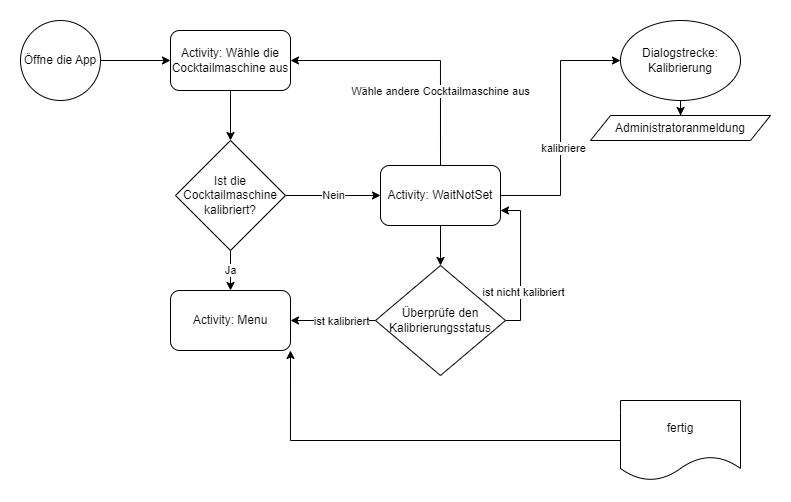
\includegraphics[scale=0.40]{Appstart.png}


\subsection{GUI: Keine Kalibrierung}
\label{subsec:nocal}

Drei mögliche Aktionen:

\begin{itemize}
\item anmelden
\item falsche Passwort: zurück in die Activity
\item und einleiten der automatischen Kalibrierung: Dialog: Kalibrierung
\item wähle eine andere Cocktailmachine aus: Cocktailmachinewahlactivity öffnet.
\item laden (Überprüfen, ob ein Admin die Kalibrierung vorgenommen hat)
\begin{itemize}

	\item Bei Erfolg (Admin hat die Kalibrierung getätigt. ): Hauptmenü öffnet
	
	\item Bei Misserfolg: Toast "Cocktailmaschine ist noch nicht bereit."

\end{itemize}
\end{itemize}


Nach der Auswahl eines der Möglichkeiten werden die Button auf nicht verfügbar gestellt, damit die Button beim Laden zwischen den Dialogen nicht angeklickt werden können.

\subsection{GUI: Dialog: Anmelden}

Dialogfenster:

Passwort angeben (''admin"). Gelange in den angemeldeten Zustand.

\subsection{GUI: Dialog: Automatische Kalibrierung}
\label{sec:dioautokal}

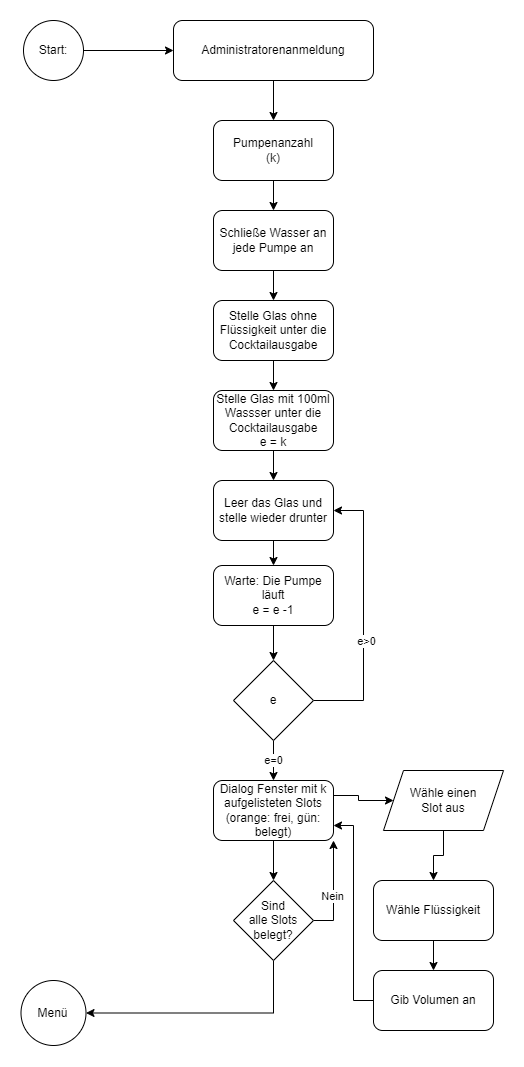
\includegraphics[scale=0.65]{calibrate.png}

\begin{enumerate}
\item Gebe die Anzahl (k) der Pumpen an.
\begin{enumerate}
	\item Toast ''Es lädt"	
\end{enumerate}
	\item Ok-Fenster: Schließe Wasser an die Pumpen.
	
	\item Ok-Fenster: Glas ohne Flüssigkeit
	
    \item Ok-Fenster: Glas mit 100ml Wassre
	
	\item Ok-Fenster: Leere das Glas
	
	\item Warte-Fenster: Pumpe läuft. k=k-1

\begin{enumerate}
		\item zu 5.: falls k>0
		
		\item zu 7.: sonst

\end{enumerate}
\item Dialog mit Liste von k Pumpen sind mit einer Slotnummer markiert und orange hinterlegt, wenn noch keine Flüssigkeit hinterlegt ist, und grün wenn eine Flüssigkeit hinterlegt ist.

\item Wähle orangene Pumpe.

\item Wähle Flüssigkeit.

\item Gibt Volumen an:
\begin{enumerate}

\item zu 7.: wenn noch nicht alle Flüssigkeiten ausgewählt wurden

\item zum Hauptmenü: sonst
\end{enumerate}
\end{enumerate}


\subsection{GUI: Darstellung Liste}
Liste von Elementen

Titel: Rezept, Zutaten, Serviervorschläge, Pumpen

Haus: Gehe zum Hauptmenü.

drehender Pfeil: Lade die Datenbank neu!

\subsubsection{Pumpen}

Statt dem Namen der Pumpen sind die Namen der zugeordneten Zutaten und die Slotnummer sichtbar.

\subsubsection{Rezepte}

Plus Zeichen: Gehe zur Erstellung eines Rezeptes.

\subsection{GUI: Anzeigen einzelner Elemente}

Für alle Elemente gilt: unter dem Titel ist ein Zeile mit drei Buttons. Der erste und linke Button ist ein Stift und öffnet die Änderungsseite für das Element. Der zweite und mittige Button ist ein drehender Pfeil. Er lädt die gesamte Datenbank neu und setzt die Seite neu auf. Der dritte und rechte Button ist eine Liste und öffnet die Liste der Elemente. Wird also eine Zutat angezeigt, so öffnet sich die Zutatenliste. Im weiteren wird von dieser Zeile als Menüzeile in der Einzelansicht gesprochen.

\subsubsection{Zutat}

Als Titel steht der Name der Zutat. Darunter kommt die Menüzeile. Unter der Menüzeile ist ein Gruppe von drei Sternen. Die Sterne haben die Farbe der Zutat. Darunter wird entweder angezeigt, dass die Zutat verfügbar oder nicht verfügbar ist. Dabei wird innerhalb einer Zeile links Ein grüner Punkt für verfügbar und dann neben der Text "verfügbar" angezeigt oder ein graues Kreuz und der Text "nicht verfügbar".

In der nächsten Zeile steht, ob die Zutat alkoholisch ist oder nicht. Dabei wird bei der Angabe alkoholisch eben der Text links angezeigt mit einem roten Warndreick auf der rechten Seite oder "nicht alkoholisch" mit einem grauen Warndreieck. Die Volumenanzeige gibt die Milliliterangabe an.

\subsubsection{Serviervorschlag}

Als Titel steht der Name des Serviervorschlags. Darunter ist die Menüzeile und da runter die Beschreibung.

\subsubsection{Pumpe}

Als Titel steht Slot und die Slotnummer. Die zugehörige Zutat wird angezeigt und das Volumen in Milliliter. Ein großer Button "Lass die Pumpe laufen".

\paragraph{Dialog: Pumpe laufen lassen}

Hier steht eine Aufforderung zur Milliliterangabe, um die Pumpe laufen zu lassen. Bei Bestätigung wird die Pumpe solange laufen gelassen.

\subsubsection{Rezepte}

Die Verfügbarkeitsanzeige ist ein grüner Punkt, wenn es verfügbar ist und rot, wenn es nicht verfügbar ist. Die Alkoholgehaltsanzeige ist ein Dreieck mit weißem Ausrufzeichen. Wenn das Dreieck rot ist, hat das Rezept alkoholische Zutaten. Wenn es grau ist, ist es nicht alkoholisch. Außerdem werden die Zutaten mit Milliliterangabe gelistet. Jede Zutat führt zur jeweiligen Zutatendarstellung. Die Serviervorschläge werden genauso gelistet. Zu letzt ist ein großer Button "Mix den Cocktail" fürt zu, Dialog: Mixen.

\paragraph{Dialog: Mixen/Activity:Simulation des Befüllens}

Beginnt mit einem CountDown mit der Anzahl der noch zu mixenden Cocktails bis zum eigenen Cocktail. Wenn der Nutzende dann dran ist, kommt die Aufforderung das eigene Glas runterzustellen, was bestätigt werden muss. Gehe zur Darstellung (Activity): Simulation des Befüllens, wenn das Mixen abgeschlossen ist, wird mit einem Dialog aufgefordert, den Cocktail abzuholen. Nach der Bestätigung des Abholens eird das Hauptmenü geöffnet.



\subsection{GUI: Ändern oder Hinzufügen}

Für alle Elemente gilt:

Möchte man ein neues Element hinzufügen. Geht man in die entsprechende Liste und wählt den Floatingbutton in der rechten unteren Ecke mit dem Plussymbol aus.

Jedes Element braucht einen Namen. Unter dem Titel gibt es ein Eingabefeld. Als Aufforderung steht in dem Feld in grauer Schrift "Füge einen Namen ein!". Wählt man das Feld aus, öffnet sich die Tastatur. Jetzt kann der Name eingegeben werden. Der eingegebene Name ist in schwarzer Schrift und nachdem ersten Einfügen eines Buchstabens ist die graue Aufforderung nicht mehr sichtbar. Handelt es sich hierbei allerdings um eine Änderung an einer bestehenden Element, dann ist zunächst die nich die Aufforderung zu sehen, sonder direkt der Name in schwarzer Schrift. Entfernt man alle Buchstaben in dem Feld, egal ob es sich um eine Änderung oder eine Neuerstellung handelt. Dann erscheint wieder die graue Aufforderung.

Unter all den Eingabefeldern. Stehen zwei Button "Abbruch" und "Speichern". Wählt man den Abbruch gelangt man in die Liste der Elementen. Wählt man den Speichervorgang. So wird die Detailansicht der neuerstellten Zutat sichtbar.

Der Speichervorgang wird abgebrochen, sollte beim Auslösen das Namensfeld leer sein.

\subsubsection{Zutat}

Daraufhin öffnet sich die AddAktivität. Der Titel heißt "Zutat".

Unter dem Namensfeld ist ein Switchbutton. Ist dieser aktiviert, steht direkt unter dem Button ein Feld "alkoholisch" mit einem roten Warndreieck davor. Ist der Button nicht aktitviert, ist das Warndreick grau und es steht "nicht alkoholisch" da. Bei der Neuerstellung ist zunächst der Switchbutton im nicht aktivenn Zustand und das Feld mit dem Warndreick ist nicht sichtbar. Erst nachdem der Nutzende mit dem Switchbutton interagierte wird die Warndreickzeile sichtbar. Bei der Änderung ist das Warndreick direkt sichtbar und der Switchbutton ist im aktiven oder inaktiven Zustand je nachdem ob die zu ändernde Zutat alkoholisch oder nicht ist.

Unter der Alkoholgehaltabfrage steht eine weitere Aufforderung "Ändere die Farbe!". Sie steht in einem Button. Wählt man diesen aus öffnet sich ein Dialog, in dem eine Farbe ausgewählt werden kann. Dieser Dialog kann abgebrochen werden mit "Abbruch". Mit dem "Speichern" wird der Zutat eine Farbe zu geordnet. Handelt es sich eine Neuerstellung und das erste Anklicken der Farbauswahl, so ist eine zufällige Farbe hinterlegt. Wurde bereits eine Farbe ausgewählt oder es ist eine Änderung, dann ist die derzeit zugeordnete Farbe der Ausgangspunkt. Der Button ändert seine Farbe mit der ausgewählten Farbe. Ist noch keine ausgewählt worden bei der Neuerstellung, so hat der Button die Standardbuttonfarbe.

\subsubsection{Serviervorschlag}

Als Titel steht "Serviervorschlag". Unter dem Namesfeld steht ein großes editierbares Textfeld. Dort steht in schwarz entweder die vorhandene Beschreibung bei einer Änderung oder in schwarz die eingegebene Beschreibung. Ist es eine Neuerstellung oder die gesamte Textfeldeingabe wurde entfernt (also die schwarzen Buchstaben), dann ist in grauen Buchstaben der Text "Füge eine Beschreibung ein." zu lesen, der so gleich wieder nicht sichtbar wird, sollte auch nur ein Buchstabe in diesem Feld eingegeben werden. Sind die Titelangabe oder die Beschreibungsangabe leer, dann wird das Speichern abgebrochen und eine Toastaufforderung zur Ergänzung angezeigt.

\subsubsection{Rezepte}

Unter dem Namensfeld steht für die Zutaten und die Serviervorschläge je eine Aufforderung des Einfügens mit einem grünen Plus daneben. Das Plus löst als Button einen Dialog aus, indem je entweder die Namen der verfügbaren Zutaten oder die der Serviervorschläge gelistet sind. Nach der Wahl einer Zutat wird in einem Dialog die Millilieterangabe gemacht und die Zutat mit Volumenangabe unter der Aufforderung hinzugelistet. Genauso sammeln sich die Namen der gewählten Serviervorschläge.

\subsubsection{Pumpe}

Es gibt kein Namensfeld. Es gibt zwei verpflichtende Felder: Ein Textfeld zur Angabe des Zutatennamens und der des Volumens. Beide müssen mit gültigen Werten ausgefüllt sein, um gespeichert zu werden.


\subsection{GUI: Menü}

Im Menü werden die wichtigsten Funktionen dem Nutzer angezeigt.
\hyperref[table:menu]{Übersicht}

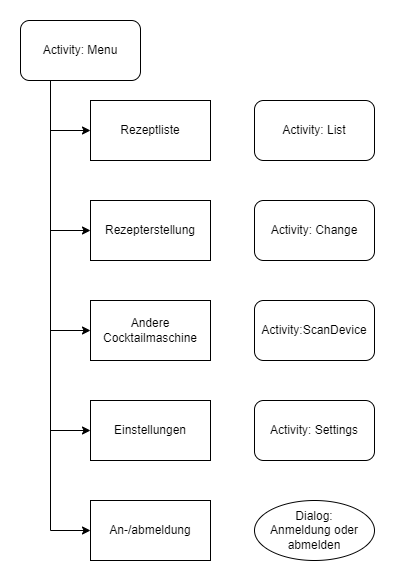
\includegraphics[scale=0.65]{Menu.png}
\captionof{figure}{Menü}


\begin{sidewaystable}[]
	\centering
	\caption{Menü}
	\label{table:menu}
	
	\begin{tabular}{|l|l|l|l|l|l|}
		\hline
		Symbol  & Nächste   & Funktion  & Sichtbar  & ausgelöste  \\
		&  Activity  &   &   &  Reaktion \\ \hline
		Liste  & ListActivity  & Liste der    & immer  & Aktivitätenwechsel \\ 
		&    &   Rezepte  &    &   \\ \hline
		Liste mit   & AddActivity  & Erstellung eines  & immer  & Aktivitätenwechsel \\ 
		Plussymbol  & AddActivity  &  neuen Rezepts  &   &  \\ \hline
		Bluetooth   & BluetoothScan  & Suche eine neue   & immer  & Aktivitätenwechsel \\
		mit Lupe  &   &  Cocktailmachine  &    &   \\ \hline
		Zahnrad  & Settingsactivity  & Einstellungs-  & immer  & Aktivitätenwechsel \\   &    & optionen   &    &   \\ \hline
		Pfeil in   & -  & Adminstratoren-  & Nur im   & Zeigen eines Anmeldedialogs, \\
		eine   &  &anmeldung   & abgemeldeten   & Wechsel in den  \\ 
		Tür   &  &    &  Zustand  & angemeldeten Zustand \\ \hline
		Pfeil aus   & -  & Adminstratoren-  & Nur im  & Wechsel in den \\  
		einer   &   &abmeldung    &  angemeldeten   & abgemeldeten  \\
		Tür  &   &    &   Zustand  &  Zustand \\ \hline
	\end{tabular}
	
\end{sidewaystable}


\subsection{GUI: Einstellung}

\subsubsection{Die Haupteinstellung:}

\hyperref[table:main]{Übersicht}
\begin{sidewaystable}[!ht]
	\centering
	\caption{Haupteinstellung}
	\label{table:main}
	\begin{tabular}{|l|l|l|l|l|}
		\hline
		\textbf{Element } & \textbf{Nächste Activity } & \textbf{Funktion } & \textbf{Sichtbar } & \textbf{ausgelöste Reaktion} \\ \hline
		Anmelden  & -  & Adminstratorenanmeldung:   & Nur im   & Funktion \\
		
		  & -  &  Zeigen eines Anmeldedialogs,   & abgemeldeten   &  \\ 
		  & -  &   Wechsel in den angemeldeten Zustand  & Zustand  &  \\ 
		 \hline
		Abmelden  & -  & Adminstratorenabmeldung:  & Nur im    & Funktion \\ 
		  & -  &  Wechsel in den abgemeldeten Zustand  & angemeldeten Zustand  &  \\ 
		  \hline
		Pumpe  & ListActivity  & Liste der Pumpen  & Nur im   & Aktivitätenwechsel \\   &   &  &  angemeldeten Zustand  &  \\ \hline
		Zutaten  & ListActivity  & Liste der verfügbaren Zutaten  & immer  & Aktivitätenwechsel \\ \hline
		Zutaten(Alle)  & ListActivity  & Liste der Zutaten  & Nur im  & Aktivitätenwechsel \\
		   &   &  &  angemeldeten Zustand  &  \\  \hline
		Rezepte  & ListActivity  & Liste der verfügbaren Rezepte  & immer  & Aktivitätenwechsel \\ \hline
		Rezepte(Alle)  & ListActivity  & Liste der Rezepte  & Nur im  & Aktivitätenwechsel \\ 
		   &   &  &  angemeldeten Zustand  &  \\ \hline
		Serviervorschläge  & ListActivity  & Liste der Serviervorschläge  & immer  & Aktivitätenwechsel \\ \hline
		Synchronisieren   & -  & Synchronisiere Rezepte  & immer  & Funktion \\ 
		 (Bluetooth)  & -  & und die Pumpen.  &   &  \\ \hline
		Scannen   & ScanActivity  & Scanne nach der   & immer  & Aktivitätenwechsel \\
		 (Bluetooth)  &   & Cocktailmaschine  &    &   \\ \hline
		Cocktailmaschinen-  & MachineSettings  & weitere   &  Nur im  & Aktivitätenwechsel \\
		-einstellung  &   &  Einstellungen  &   angemeldeten Zustand  &  \\
		 \hline
		Komplett neuladen  & -  & Synchronisiere Pumpenstand  & immer  & Funktion \\
		 (Datenbank)  &   &  und damit die Verfügbarkeit.  &    &  \\  \hline
		Füge vorbereitete  & -  & Lade Rezepte aus   & immer  & Funktion \\
		Rezepte hinzu   &   &Json und CSV-Dateien.  &    &   \\ 
		(Datenbank)  &   &   &    &   \\  \hline
	\end{tabular}
\end{sidewaystable}

\subsubsection{Die Cocktailmaschineneinstellungen:}
(Erreichbar nur im \textbf{an}gemeldeten Zustand)
\hyperref[table:mach]{Übersicht}

\begin{sidewaystable}[!ht]
	\centering
	\label{table:mach}
	\caption{Cocktailmaschineneinstellungen}
	\begin{tabular}{|l|l|l|l|}
		\hline
		\textbf{Element } & \textbf{Nächste Activity } & \textbf{Funktion } & \textbf{ausgelöste Reaktion} \\ \hline
		Neukalibrierung   & WaitNotSet  & Setze die Kalibrierung zurück   & Aktivitätenwechsel \\
		 (Kalibrierung)  &   &  und kalibriere die Cocktailmaschine neu.  &  \\
		   &   &  Geh zu WaitNotSet.  &  \\ \hline
		Waagenkalibrierung   & ScaleSettingsActivity  & weitere   & Aktivitätenwechsel \\ 
		 (Kalibrierung)  &   &  Einstellungen  &  \\ \hline
		Pumpenkalibrierung   & PumpSettingsActivity  & weitere   & Aktivitätenwechsel \\
		(Kalibrierung)  &   &  Einstellungen  &  \\ \hline
		Statusabfrage   & -  & Zeige in einem Dialog  & Funktion \\
		 (Zustand)  &   &den derzeitigen Zustand an,   &  \\ 
		   &   &  wie von Freya beschrieben.  &  \\ \hline
		Reinigung (Zustand)  & -  & Schickt Reinigungsbefehl  & Funktion \\ \hline
		Neustart & -  & Schickt Neustartbefehl.  & Funktion \\ 
		(Neustart)     &  & (Kein Zurücksetzen!)  &  \\ \hline
		Werkseinstellungen   & WaitNotSet  & Setze die Kalibrierung zurück.  & Aktivitätenwechsel \\
		 (Neustart)  &    &  Geh zu WaitNotSet.  &   \\ \hline
	\end{tabular}
\end{sidewaystable}



\subsubsection{Die Waagenkalibrierung:}
(Erreichbar nur im \textbf{an}gemeldeten Zustand)
\hyperref[table:weight]{Übersicht}
\begin{sidewaystable}[!ht]
	\centering
	\label{table:weight}
	\caption{Waagenkalibrierung}
	\begin{tabular}{|l|l|l|l|}
		\hline
		\textbf{Element } & \textbf{Nächste Activity } & \textbf{Funktion } & \textbf{ausgelöste Reaktion} \\ \hline
		Kalibriere  & -  & Setze das Gewicht mit Hilfe eines  & Funktion \\
		   &    & Dialogs. Schicke Gewichtsangabe.  &   \\ \hline
		Tariere  & -  & Schicke Tarierungsbefehl.  & Funktion \\ \hline
		Skaliere  & -  & Setze Saklierungsfaktor mit des Dialogs.  & Funktion \\ \hline
		derzeitges    & -  & Zeige in einem Dialog   & Funktion \\
		 Gewicht  &    & das derzeitiges Gewicht an.  &   \\ \hline
	\end{tabular}
\end{sidewaystable}

\subsubsection{Die Pumpenkalibrierung:}
(Erreichbar nur im \textbf{an}gemeldeten Zustand)
\hyperref[table:pump]{Übersicht}
\begin{sidewaystable}[!ht]
	\centering
	\label{table:pump}
	\caption{Pumpenkalibrierung}
	\begin{tabular}{|l|l|l|l|}
		\hline
		\textbf{Element } & \textbf{Nächste Activity } & \textbf{Funktion } & \textbf{ausgelöste Reaktion} \\ \hline
		Automatische   & WaitNotSet  & Setze die Kalibrierung zurück und  & Aktivitätenwechsel \\
		 Kalibrierung  &   & kalibriere die Cocktailmaschine neu.   &  \\ 
		   &   & Geh zu WaitNotSet.  &  \\ \hline
		Setze Pumpzeiten  & -  & Dialog mit vier Eingabefeldern:   &  \\	
		 (Kalibrierung)  & -  &  Zeit1, Zeit2, Volumen1, Volumen2,   &  \\
		   & -  &  wie von Freya beschrieben.  &  \\
		   & -  &  Wird für alle Pumpen gleichzeitig verwendet.  &  \\ \hline
	\end{tabular}
\end{sidewaystable}




\subsection{Datenbank}

Die Datenbank verwendet die von Android zur Verfügung stehende Standardimplementierung. 
 
Die Datenbank ist über ein paar simplen Designentscheidungen implementiert. 


\subsection{DB: Zustände}
\label{sec:dbstatus}

Es gibt mehrere \hyperref[sec:status]{Zustände}, die die Cocktailmaschine ein nehmen kann. Programmtechnisch ist es sinnvoll diese in Enums zu verpacken, wobei es mehrere Enum-Pakete gibt. Die \hyperref[sec:statusrez]{Standardzustände}, wie das Mixen eines Cocktails und die \hyperref[sec:statuscal]{Zustände während bzw. kurz vor der Kalibrierung} und die auftretenden \hyperref[sec:statuserror]{Fehler}. In den Enums werden alle Zustände gelistet und die Bluetoothabfrage und die Anzeige via eines Dialogs ermöglicht.

\subsection{DB: Administrator}

Es gibt neben den \hyperref[sec:dbstatus]{ESP-Zustände} noch einen weiteren App internen Zustand und zwar den des Nutzers. Dieser kann ein "User" oder ein "Admin" sein, wobei "Admin" die Abkürzung für Administrator ist. Innerhalb der App wird nach der Anmeldung des Nutzers die erweiterten Funktionen freigeschaltet, wie die Kalibrierung der Maschine. 

\subsection{Schnittstellen}

Es gibt 5 Hauptschnittstellen, eine für Pumpen, für die Rezepte, die Zutaten, die Serviervorschläge und die Cochtailmaschine selbst. 
Die ersten vier Komponenten von Pumpen, Rezepten, Zutaten und Seviervorschläge ähneln sich. Die Schnittstelle dient als Dateiformat für ein einzelnes Objekt wie ein Rezept mit Namen, Zutaten und ID oder in statischen Funktionen zur Abfrage der Datenbank. Finde zum Beispiel alle Zutaten, die "Wod" im Namen tragen. Die Schnittstelle der Cocktailmaschine diente zunächst als Dummy für die Bluetoothverbindung, weil diese noch nicht implementiert war und trotzdem aufgerufen werden sollte, um die GUI die Cocktailmaschienenfunktionen simulieren zu lassen und diente im Anschluss als Oberfläche die Bluetoothverbindung einzelner \hyperref[sec:espbefehle]{Cocktailmaschinenfunktionen} zu erstellen, sowie die \hyperref[sec:dioautokal]{automatische Kalibrierung} zu starten. Dabei ist zum Beispiel die Anmeldung oder der Start des Reinigungsprogramms eine Variante.
